\fancyhead[LH]{\zihao{-5}{\songti 重庆大学本科学生毕业论文（设计）}}
\fancyhead[RH]{\zihao{-5}{\songti 4\quad 实验}}

\section{实验}
\subsection{图表格式}
\zihao{-4} 
本章将主要介绍一些图表和公式的格式...\\

\begin{figure}[htb] 
\center{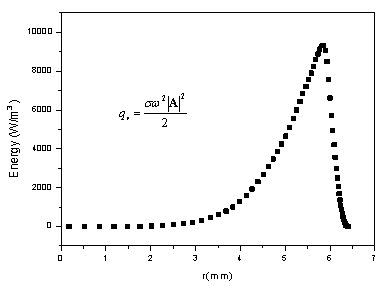
\includegraphics[width=0.95\textwidth]  {img/fig2.png}} 
\caption{内热源沿径向的分布}
\end{figure} %图表上下各空一行

\begin{table}[htbp]
\centering
\caption{高频感应加热的基本参数}
\small
\begin{tabular}{c c c c}
\toprule
感应频率 &感应发生器功率 & 工件移动速度  &感应圈与零件间隙\\
（KHz）&($\% \times$80Kw) &(mm/min)  &(mm)\\
\midrule
250 &88 &5900 &1.65\\

250 &88 &5900 &1.65\\

250 &88 &5900 &1.65\\

250 &88 &5900 &1.65\\



\bottomrule
\end{tabular}
\end{table}



\begin{table}[htbp]
\centering
\captionsetup{singlelinecheck=off}
\caption*{续表3.1}
\small
\begin{tabular}{c c c c}
\toprule
感应频率 &感应发生器功率 & 工件移动速度  &感应圈与零件间隙\\
（KHz）&($\% \times$80Kw) &(mm/min)  &(mm)\\
\midrule
250 &88 &5900 &1.65\\

250 &88 &5900 &1.65\\
\bottomrule
\end{tabular}
\end{table}
\vspace{\baselineskip}
%表格太大需要转页时，需要在续表上方注明“续表”，表头也应重复排出。


\subsection{公式格式}


\begin{eqnarray}
\frac{1}{\mu} \nabla^2A - j \omega \sigma A -\nabla(\frac{1}{\mu}) \times(\nabla \times A)+J_0=0
\end{eqnarray}


\subsection{本章小结}
\zihao{-4} 
本章介绍\cite{hassan2022vivisecting}了……

